\documentclass{standalone}
\usepackage{tikz}
\usepackage{ctex,siunitx,ninecolors}
\setCJKmainfont{Noto Serif CJK SC}
\usepackage{tkz-euclide}
\usepackage{amsmath}
\usetikzlibrary{patterns, calc}
\usetikzlibrary {decorations.pathmorphing, decorations.pathreplacing, decorations.shapes,}
\begin{document}
\small
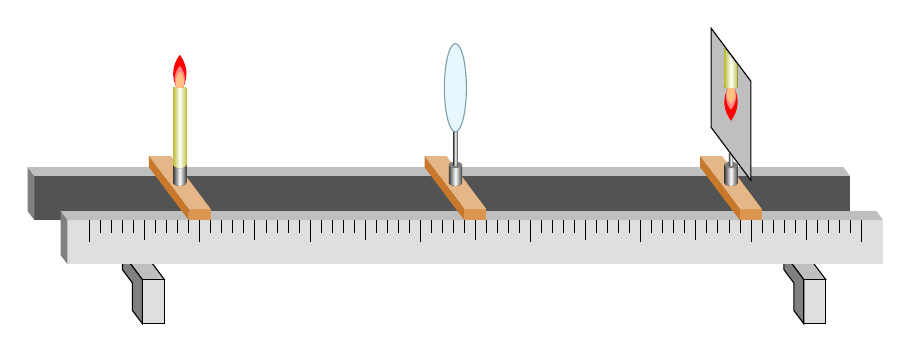
\begin{tikzpicture}[>=latex,scale=1.4]
  \foreach \x in {0.3,6.3}
  {
    \begin{scope}[xshift=\x cm,yshift=-0.3cm]
      \draw[fill=lightgray](0,0)--(0.18,-0.24)--++(0.2,0)--++(-0.18,0.24)--cycle;
      \draw[fill=lightgray!50](0.18,-0.24)rectangle++(0.2,-0.4);
      \draw[fill=gray](0,0)--(0.18,-0.24)--++(0,-0.4)--++(-0.09,0.12)--++(0,0.25)--++(-0.09,0.12)--cycle;
    \end{scope}
  }
  \begin{scope}[xshift=-0.3cm,yshift=0.4cm]
    \fill[darkgray!90](-0.2,0)rectangle(7.2,-0.4);
    \fill[gray](-0.2,0)--(-0.2,-0.4)--++(-0.06,0.08)--++(0,0.4)--cycle;
    \fill[lightgray](-0.2,0)--++(-0.06,0.08)--++(7.4,0)--++(0.06,-0.08)--cycle;
  \end{scope}
  \begin{scope}
    \fill[lightgray!50](-0.2,0)rectangle(7.2,-0.4);
    \fill[gray](-0.2,0)--(-0.2,-0.4)--++(-0.06,0.08)--++(0,0.4)--cycle;
    \fill[lightgray](-0.2,0)--++(-0.06,0.08)--++(7.4,0)--++(0.06,-0.08)--cycle;
    \foreach \x in {0,1,...,6}
    {
      \draw[very thin](\x,0)--(\x,-0.2);
      \draw[very thin](\x+0.5,0)--(\x+0.5,-0.18);
      \foreach \y in {1,2,3,4,6,7,8,9}
      {
        \draw[very thin](\x+0.1*\y,0)--++(0,-0.12);
      }
    }
    \draw[very thin](7,0)--(7,-0.2);
  \end{scope}
  \begin{scope}[xshift=1cm]
    \fill[brown7](-0.1,0)rectangle(0.1,0.1);
    \fill[brown8](-0.1,0.1)--(0.1,0.1)--++(-0.36,0.48)--++(-0.2,0);
    \fill[brown6](-0.1,0)--(-0.1,0.1)--++(-0.36,0.48)--++(0,-0.1);
    \fill[left color=darkgray,right color=darkgray,middle color=white](-0.18,0.34)ellipse(0.06 and 0.03);
    \fill[left color=darkgray,right color=darkgray,middle color=white](-0.24,0.34)rectangle++(0.12,0.16);
    \fill[left color=yellow!50!gray,right color=yellow!50!gray,middle color=white](-0.18,0.5)ellipse(0.06 and 0.03);
    \fill[left color=yellow!50!gray,right color=yellow!50!gray,middle color=white](-0.24,0.5)rectangle++(0.12,0.7);
    \fill[red](-0.15,1.2)to[bend right](-0.18,1.5)to[bend right](-0.21,1.2);
    \fill[red!50](-0.15,1.2)to[bend right](-0.18,1.4)to[bend right](-0.21,1.2);
    \fill[orange!50](-0.15,1.2)to[bend right](-0.18,1.35)to[bend right](-0.21,1.2);
  \end{scope}
  \begin{scope}[xshift=3.5cm]
    \fill[brown7](-0.1,0)rectangle(0.1,0.1);
    \fill[brown8](-0.1,0.1)--(0.1,0.1)--++(-0.36,0.48)--++(-0.2,0);
    \fill[brown6](-0.1,0)--(-0.1,0.1)--++(-0.36,0.48)--++(0,-0.1);
    \fill[left color=darkgray,right color=darkgray,middle color=white](-0.18,0.34)ellipse(0.06 and 0.03);
    \fill[left color=darkgray,right color=darkgray,middle color=white](-0.24,0.34)rectangle++(0.12,0.16);
    \fill[gray](-0.18,0.5)ellipse(0.06 and 0.03);
    \fill[left color=darkgray,right color=darkgray,middle color=white](-0.18,0.5)ellipse(0.02 and 0.01);
    \fill[left color=darkgray,right color=darkgray,middle color=white](-0.20,0.5)rectangle++(0.04,0.3);
    \draw[fill=cyan!30,fill opacity=0.3,draw=cyan!30!gray](-0.18,1.2)ellipse(0.1 and 0.4);
  \end{scope}
  \begin{scope}[xshift=6cm]
    \fill[brown7](-0.1,0)rectangle(0.1,0.1);
    \fill[brown8](-0.1,0.1)--(0.1,0.1)--++(-0.36,0.48)--++(-0.2,0);
    \fill[brown6](-0.1,0)--(-0.1,0.1)--++(-0.36,0.48)--++(0,-0.1);
    \fill[left color=darkgray,right color=darkgray,middle color=white](-0.18,0.34)ellipse(0.06 and 0.03);
    \fill[left color=darkgray,right color=darkgray,middle color=white](-0.24,0.34)rectangle++(0.12,0.16);
    \fill[gray](-0.18,0.5)ellipse(0.06 and 0.03);
    \fill[left color=darkgray,right color=darkgray,middle color=white](-0.18,0.5)ellipse(0.02 and 0.01);
    \fill[left color=darkgray,right color=darkgray,middle color=white](-0.20,0.5)rectangle++(0.04,0.1);
    \draw[fill=lightgray](-0.18,0.6)--++(-0.18,0.24)--++(0,0.9)--++(0.36,-0.48)--++(0,-0.9)--cycle;
    \fill[red](-0.15,1.2)to[bend left](-0.18,0.9)to[bend left](-0.21,1.2);
    \fill[red!50](-0.15,1.2)to[bend left](-0.18,1.0)to[bend left](-0.21,1.2);
    \fill[orange!50](-0.15,1.2)to[bend left](-0.18,1.05)to[bend left](-0.21,1.2);
    \fill[left color=yellow!50!gray,right color=yellow!50!gray,middle color=white](-0.24,1.2)--(-0.12,1.2)--(-0.12,1.4)--++(-0.12,0.16);
  \end{scope}
\end{tikzpicture}
\end{document}